\documentclass[10pt,a4paper]{article}
\usepackage[a4paper,margin=0.75cm]{geometry}
\usepackage[utf8]{inputenc}
\usepackage[T1]{fontenc}
\usepackage{titlesec}
\usepackage{enumitem}
\usepackage[hidelinks]{hyperref}
\usepackage{fancyhdr}
\usepackage{multicol}
\usepackage{xcolor}
\usepackage{graphicx}

\definecolor{accentTitle}{HTML}{0E6E55}
\definecolor{accentText}{HTML}{0E6E55}
\definecolor{accentLine}{HTML}{A16F0B}
\definecolor{muted}{HTML}{666666}

\pagestyle{fancy}\fancyhf{}
\renewcommand{\headrulewidth}{0pt}
\renewcommand{\footrulewidth}{0pt}

\hypersetup{pdfauthor={Oualid Hmoudou},pdftitle={CV - Oualid Hmoudou - Developpeur},pdfsubject={Curriculum Vitae}}

\titleformat{\section}{\vspace{-4pt}\color{accentText}\raggedright\large\bfseries}{}{0em}{}[\color{accentLine}\titlerule]
\newenvironment{resume_list}{\vspace{-2pt}\begin{itemize}[itemsep=0.3pt,parsep=0pt,topsep=0.3pt,leftmargin=18pt]}{\end{itemize}\vspace{-2pt}}
\setlist[itemize]{label=\textbullet}
\newcommand{\heading}[2]{{\raggedright\noindent\textbf{#2} \quad \textbf{#1}\\}}

\setlength{\parskip}{0.5pt}
\raggedbottom\raggedright\urlstyle{same}

\begin{document}
\vspace*{-10pt}

% ── Header ──────────────────────────────────────────────────────────────────
\noindent
\begin{minipage}[t]{0.22\textwidth}\vspace{6pt}
  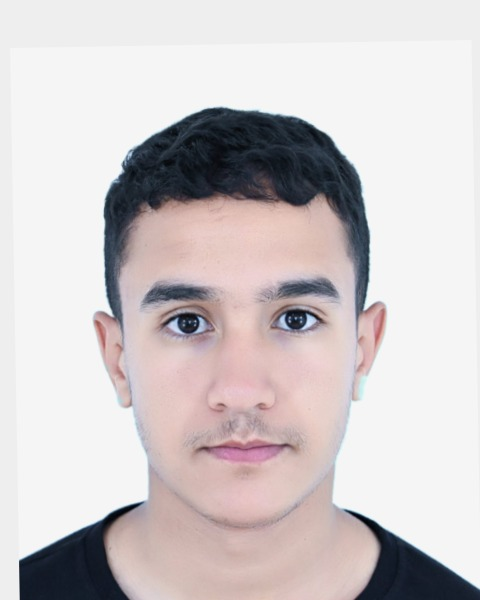
\includegraphics[width=2.5cm,height=3.3cm,keepaspectratio]{myphoto.jpeg}
\end{minipage}\hfill
\begin{minipage}[t]{0.76\textwidth}
  \begin{center}
    {\Huge\color{accentTitle} OUALID HMOUDOU}\\[4pt]
    {\color{accentLine}\hrule}\vspace{3pt}
    {\small
      +33\,6\,20\,24\,42\,27 \quad|\quad
      \href{mailto:oualidhmoudou@gmail.com}{oualidhmoudou@gmail.com} \quad|\quad
      Amiens, France \quad|\quad Permis B
    }\\[2pt]
    {\small
      \textbf{Portfolio : }\href{https://oualidhmoudou.github.io}{\color{accentText}\underline{oualidhmoudou.github.io}}
      \quad|\quad
      \href{https://linkedin.com/in/oualid-hmoudou-16880a225}{\color{accentText}\underline{LinkedIn}}
    }\\[2pt]
    {\color{accentLine}\hrule}
  \end{center}
\end{minipage}
\vspace{1pt}\centering\small\color{muted}
Étudiant Master MIAGE (M1) --- \textbf{Développeur Web Fullstack} --- Alternance dès septembre 2026\par
\vspace{3pt}\raggedright

% ── Profil ──────────────────────────────────────────────────────────────────
\section{Profil}
Développeur web fullstack en Master MIAGE à l'UPJV d'Amiens, à l'aise sur l'ensemble du cycle de vie applicatif : analyse des besoins, conception d'\textbf{API REST}, modélisation de bases de données, développement et déploiement. Pratique solide du développement côté serveur (\textbf{PHP / Symfony}, Laravel) comme d'écosystèmes complémentaires (C\#/.NET, Vue.js), avec une exigence constante de qualité (tests, revue de code, Git). Autonome, rigoureux et curieux des enjeux métier.

% ── Compétences ─────────────────────────────────────────────────────────────
\section{Compétences techniques}
\begin{multicols}{2}
\begin{itemize}[itemsep=0.3pt,leftmargin=18pt]
  \item \textbf{Backend \& Web} : PHP, Symfony, Laravel, C\#/.NET, Node.js, API REST
  \item \textbf{Frontend} : JavaScript, Vue.js, React, HTML/CSS, Bootstrap
  \item \textbf{Bases de données} : MySQL, PostgreSQL, Oracle ; SQL avancé, modélisation
  \item \textbf{Architecture \& qualité} : Clean Architecture, SOLID, design patterns, tests unitaires, revue de code
  \item \textbf{DevOps \& outils} : Git/GitLab, GitHub Actions, Docker, Linux, Maven
  \item \textbf{Méthodes} : Agile/Scrum, analyse des besoins, documentation technique
\end{itemize}
\end{multicols}

% ── Expériences ─────────────────────────────────────────────────────────────
\section{Expériences professionnelles}

\heading{Teatch, Paris \textbf{--} Stage Product Engineer (Développement Fullstack)}{Avr. -- Juin 2026}
\begin{resume_list}
  \item Refonte complète d'une plateforme web (front \& back) : conception des composants, design d'\textbf{API REST}, modélisation de la base de données.
  \item Intégration de fonctionnalités d'\textbf{IA} pour automatiser des processus métier.
  \item Pratiques de qualité : versioning Git, tests unitaires, revue de code, déploiement.
\end{resume_list}

\heading{ORMVAH, Marrakech \textbf{--} Développeur Web \& Assistant Chef de Projet}{Avr. -- Juin 2023}
\begin{resume_list}
  \item Conception et développement d'une application web de gestion sous \textbf{Laravel} ; modélisation et optimisation du schéma \textbf{MySQL} (requêtes complexes, vues, procédures stockées).
  \item Recette, déploiement, formation des utilisateurs finaux et rédaction de la documentation technique.
\end{resume_list}

\heading{NJT Group \textbf{--} Développeur Web (Stage)}{Juin -- Août 2022}
\begin{resume_list}
  \item Développement from scratch d'une application de gestion des formations (\textbf{PHP}, \textbf{MySQL}) : modélisation de la base, modules métier et tableaux de bord de suivi.
\end{resume_list}

\heading{EPSF, Amiens \textbf{--} Stage Analyste BI}{Depuis juin 2026}
\begin{resume_list}
  \item Tableaux de bord décisionnels et automatisation de reportings (Power BI, DAX, SQL).
\end{resume_list}

% ── Formation ───────────────────────────────────────────────────────────────
\section{Formations}
\begin{resume_list}
  \item \textbf{2025 -- En cours} \quad \textbf{Master MIAGE} (M1) -- Université de Picardie Jules Verne, Amiens
  \item \textbf{2023 -- 2025} \quad \textbf{Licence Informatique} -- Université de Picardie Jules Verne, Amiens
  \item \textbf{2021 -- 2023} \quad \textbf{DUT Génie Informatique} -- EST Essaouira, Maroc
\end{resume_list}

% ── Projets ─────────────────────────────────────────────────────────────────
\section{Projets significatifs}
\begin{resume_list}
  \item \textbf{Plateforme de Billetterie en ligne} (C\#/.NET 8, Vue.js 3, API REST, MySQL) --- application fullstack en équipe Agile/Scrum : modélisation BDD, API documentée (Swagger), intégration front/back, pipeline CI/CD GitHub Actions.
  \item \textbf{Gestion d'Association Universitaire} (\textbf{Laravel}) --- application web complète en tant que chef de projet : planification des sprints, livraisons, documentation et formation des utilisateurs.
  \item \textit{Autres réalisations (Clean Architecture .NET, multithreading Java, IA Q-learning…) détaillées sur le \href{https://oualidhmoudou.github.io}{\color{accentText}\underline{portfolio}}.}
\end{resume_list}

% ── Langues & Engagement ────────────────────────────────────────────────────
\vspace{1pt}
\begin{minipage}[t]{0.48\textwidth}
\section{Langues}
\begin{resume_list}
  \item \textbf{Français} : C1 \quad \textbf{Anglais} : C1
  \item \textbf{Arabe} : natif \quad \textbf{Espagnol} : A1
\end{resume_list}
\end{minipage}\hfill
\begin{minipage}[t]{0.48\textwidth}
\section{Engagement}
\begin{resume_list}
  \item \textbf{Croix-Rouge Française} -- Équipier Secouriste (depuis mars 2024)
\end{resume_list}
\end{minipage}

\end{document}
